\documentclass{article}
\usepackage[margin=1in]{geometry}
\usepackage{amsmath,amsthm,amssymb}
\usepackage{bbm,enumerate,mathtools}
\usepackage{tikz,pgfplots}
\usepackage{chessboard}
\usepackage[hidelinks]{hyperref}
\usepackage{multicol} % Problem 35
\usepackage{xstring} % Difficulty command
\usetikzlibrary{shapes.geometric}

\newenvironment{question}{\begin{trivlist}\item[\textbf{Question.}]}{\end{trivlist}}
\newenvironment{note}{\begin{trivlist}\item[\textbf{Note.}]}{\end{trivlist}}
\newenvironment{references}{\begin{trivlist}\item[\textbf{References.}]}{\end{trivlist}}
\newenvironment{related}{\begin{trivlist}\item[\textbf{Related.}]\end{trivlist}\begin{enumerate}}{\end{enumerate}}

\newcommand\score[1]{
\pgfmathsetmacro\pgfxa{#1+1}
\tikzstyle{scorestars}=[
  star,
  star points=5,
  star point ratio=2.25,
  draw,
  inner sep=3pt,
  anchor=outer point 5
]
  \begin{tikzpicture}[baseline]
    \draw[opacity=0] (0,-0.5) rectangle (0,0.2); % Workaround for whitespace at the bottom.
    \foreach \i in {1,...,4} {
      \pgfmathparse{(\i<=#1?"yellow":"gray")}
      \edef\starcolor{\pgfmathresult}
      \draw (\i*4.5ex,0) node[name=star\i,scorestars,fill=\starcolor]  {};
    }
  \end{tikzpicture}
}

\newcommand{\difficulty}[1]{%
  \IfEqCase{#1}{%
      {1}{
        
\begin{tikzpicture}[scale=0.7, baseline=0.9mm]%
          \definecolor{slopegreen}{rgb}{0.0, 0.5, 0.0}%
          \fill[slopegreen] (0.5,0.5) circle (0.5);%
        \end{tikzpicture}%
      }%
      {2}{
        
\begin{tikzpicture}[scale=0.7, baseline=0.9mm]%
          \definecolor{slopeblue}{rgb}{0.0, 0.44, 1.00}
          \fill[slopeblue] (0,0) rectangle (1,1);%
        \end{tikzpicture}%
      }%
      {3}{
\begin{tikzpicture}[scale=0.7, baseline=0.9mm]\fill (0,0.5)--(0.5, 0)--(1,0.5)--(0.5,1)--cycle; \end{tikzpicture}}%
      {4}{
\begin{tikzpicture}[scale=0.7, baseline=0.9mm]\fill (0.25,0)--(0,0.5)--(0.25,1)--(0.5,0.5)--cycle; \fill (0.75,0)--(0.5,0.5)--(0.75,1)--(1,0.5)--cycle;\end{tikzpicture}}%
      % you can add more cases here as desired
  }[\PackageError{difficulty}{Undefined difficulty level: #1}{}]%
}%
\newcommand{\rating}[2]{\difficulty{#1}\\\score{#2}\\}


\begin{document}
\rating{3}{2}
  Consider convex polygons with integer vertices and minimal area.

\begin{figure}[ht!]
  \centering
  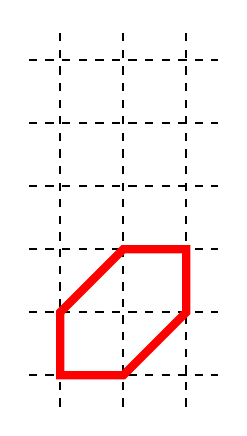
\begin{tikzpicture}[scale=0.8]
    \draw[dashed, thick] (-0.5,-0.5) grid (2.5,5.5);
    \draw[line width=3, red] (0,0)--(0,1)--(1,2)--(2,2)--(2,1)--(1,0)--cycle;
  \end{tikzpicture}
  ~~~
  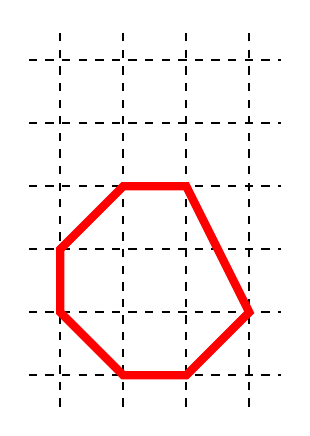
\begin{tikzpicture}[scale=0.8]
    \draw[dashed, thick] (-0.5,-0.5) grid (3.5,5.5);
    \draw[line width=3, red] (0,1)--(0,2)--(1,3)--(2,3)--(3,1)--(2,0)--(1,0)--cycle;
  \end{tikzpicture}
  ~~~
  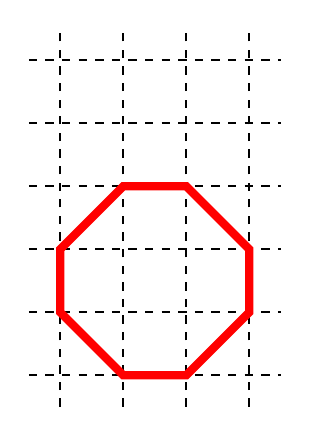
\begin{tikzpicture}[scale=0.8]
    \draw[dashed, thick] (-0.5,-0.5) grid (3.5,5.5);
    \draw[line width=3, red] (0,1)--(0,2)--(1,3)--(2,3)--(3,2)--(3,1)--(2,0)--(1,0)--cycle;
  \end{tikzpicture}
  ~~~
  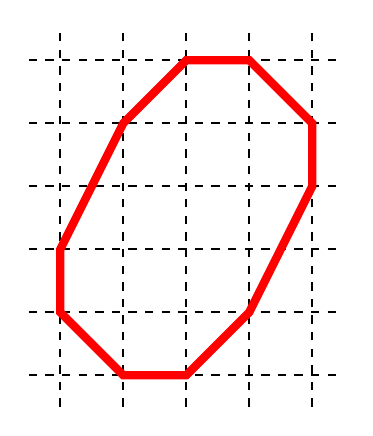
\begin{tikzpicture}[scale=0.8]
    \draw[dashed, thick] (-0.5,-0.5) grid (4.5,5.5);
    \draw[line width=3, red] (0,1)--(0,2)--(1,4)--(2,5)--(3,5)--(4,4)--(4,3)--(3,1)--(2,0)--(1,0)--cycle;
  \end{tikzpicture}
  \caption{
    Candidates for minimal area $6, 7, 8$ and $10$-gons.
  }
\end{figure}

\begin{question}
  What is the minimal area of a convex lattice $n$-gon.
\end{question}

\begin{related}
  \item What if the sum of side lengths is minimized instead? Measured via the
  taxicab metric?
  \item What if the polygons are minimized with respect to the height/width of
  the smallest grid? Or the number of complete cells they contain? (e.g. the
  examples contain 0, 4, 5, and 10 cells respectively) The number of partial
  cells they contain? (e.g. 4, 9, 9, 18) respectively?
  \item What if the polygons can be concave?
  \item What if the concave polygons cannot have any acute angles?
  \item What if the concave polygons can be decomposed into polyabolos?
  \item What if the polygons must have $180^\circ$ or horizontal symmetry?
\end{related}

\begin{references}
  \item \url{https://en.wikipedia.org/wiki/Polyabolo}
  \item Problem 5, Problem 7, and Problem 88.
\end{references}

\end{document}
